\chapter{Establishing Benchmark of Physics-based PMP Estimation using A Hybrid Approach: Supplemental Materials}


This appendix includes the supplemental materials for chapter \ref{ch:WRR}. As the time of writing the dissertation, these materials have been under review for the \textit{Water Resources Research}.

\bigbreak

\noindent
\hangafter=1
\setlength{\hangindent}{2em}
Chen, X., Hossain, F., and Leung, R. L., Probable maximum precipitation in the U.S. Pacific Northwest in a changing climate. \textit{Water Resources Research} (under review).

\vspace{10mm}

\noindent

\section{Figures}

\begin{figure}[htbp]
	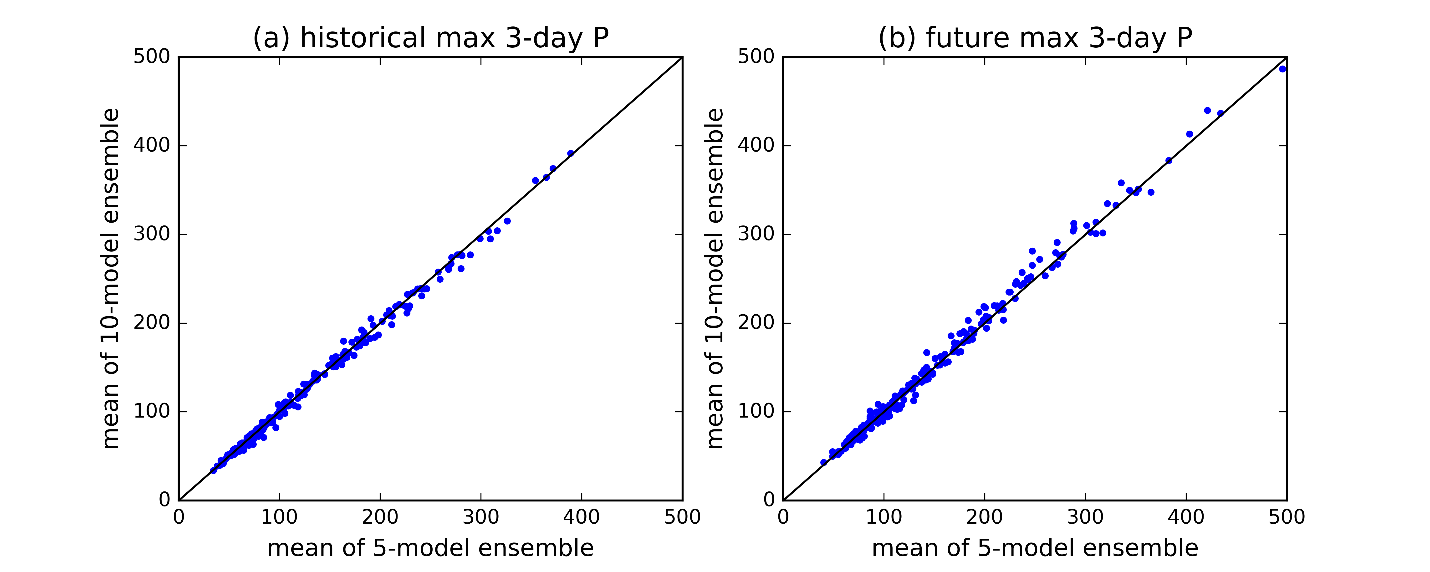
\includegraphics[width=\linewidth]{pics/ch5/figS1.png}
	\caption{Comparison of 5-model and 10-model ensemble mean estimation of maximum 3-day precipitation in the 220 Hydrological Unit (HU). Panel (a) is the historical estimation (1970-2016), (b) is the future estimation (2050-2099). The x-axis shows the 5-model ensemble mean, and the y-axis shows the 10-model ensemble. Black lines are the 1:1 lines.}
	\label{fig:5-S1}
\end{figure}

\begin{figure}[htbp]
	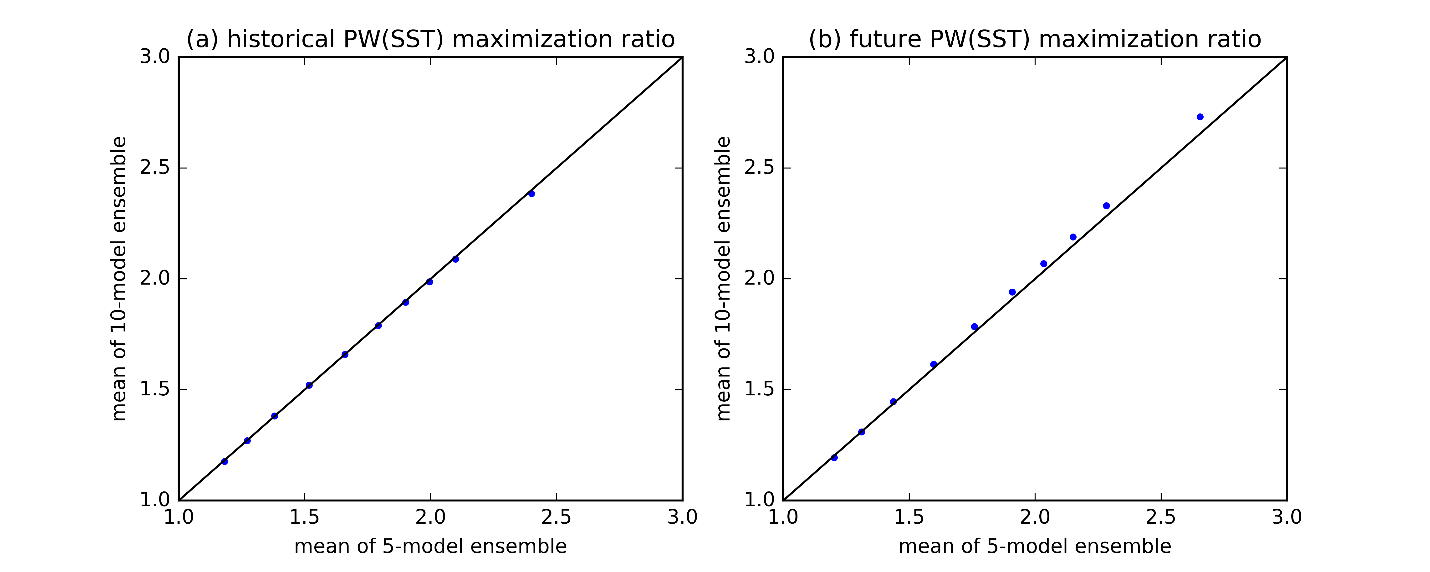
\includegraphics[width=\linewidth]{pics/ch5/figS2.png}
	\caption{Comparison of 5-model and 10-model ensemble mean estimation of average moisture maximization ratios in the box ocean region. Panel (a) is the historical estimation (1970-2016), (b) is the future estimation (2050-2099). The x-axis shows the 5-model ensemble mean, and the y-axis shows the 10-model ensemble. Black lines are the 1:1 lines. Box ocean region is defined as the ocean area between $15^{\circ}$N-$55^{\circ}$N and $180^{\circ}$W-PNW coast.}
	\label{fig:5-S2}
\end{figure}

\begin{figure}[htbp]
	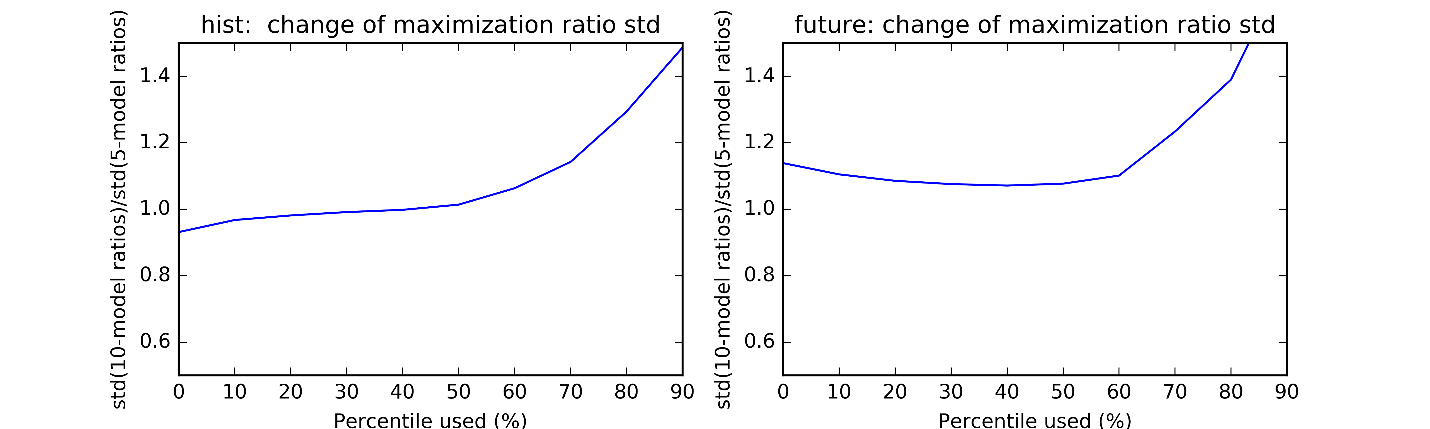
\includegraphics[width=\linewidth]{pics/ch5/figS3.png}
	\caption{Relationship between $Var10(maximization ratio)$ and $Var5(maximization ratio)$. Panel (a) is the historical ratio, (b) is the future ratio. x-axis is the various percentile from 0\% to 90\%, and y-axis is $Var10(maximization ratio)/Var5(maximization ratio)$ for a given percentile. For historical storms, $Var10/Var5$ can be taken as 1 (100\%), while for future storms, $Var10/Var5$ can be taken as 1.1 (110\%).}
	\label{fig:5-S3}
\end{figure}